
%matplotlib inline: esto es para que las graficas aparescan a dentro.

\documentclass{article}
%Reporte de computacional
%matplotlib inline: esto es para que las graficas aparescan a dentro.
\usepackage{hyperref}
\usepackage{amsmath}
\usepackage{amsthm}
\usepackage{amssymb}
\usepackage{graphicx}
\usepackage{ifxetex}
\ifxetex
\usepackage{fontspec}
\else
\usepackage[T1]{fontenc}
\usepackage[utf8]{inputec}
\usepackage{lmodern}
\fi



\begin{document}
\title{El Atractor de Lorenz }
\author{Ramses Pacheco Ortiz}
\date{26 de Abril Del 2018}
\maketitle  


\section{Introducción}

Esta es la segunda evaluacion realizada en este cursos, en donde se practicaron los conocimientos adquieridos en las actividades 6,7,8.


Esta actividad concistió en describir un sistema de ecuaciones para realizar una animacion y visualizacion de un efecto llamado Atractor de Lorenz con ayuda de ejemplo brindado por el maestro.


Esta actividad fue llevada acabo con python con la ayuda de jupyter lab y sus bibliotecas(numpy,pyplot,integrate,etc.).
Dicha actividad consistio en 4 puntos que mas adelante trataremos y se mostraran sus respectivas graficas.


A continuación se proporcionara un breve descripcion del sistema estudiado:

El atractor de Lorenz. Es un concepto introducido por Edward Lorenz en 1963; es un sistema dinámico determinista tridimensional no lineal derivado de las ecuaciones simplificadas de rollos de convección que se producen en las ecuaciones dinámicas de la atmósfera terrestre. 


\section{Procedimiento}

El primer punto consistió en reproducir el ejemplo, brindado por el profesor y ver las graficas que se producieron.
Este codigo incluia los sigueintes parametros:

\begin{center}
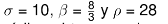
\includegraphics[height=1cm]{cod1.png}
\end{center}


con los cuales se producieron las graficas siguientes:

\begin{center}
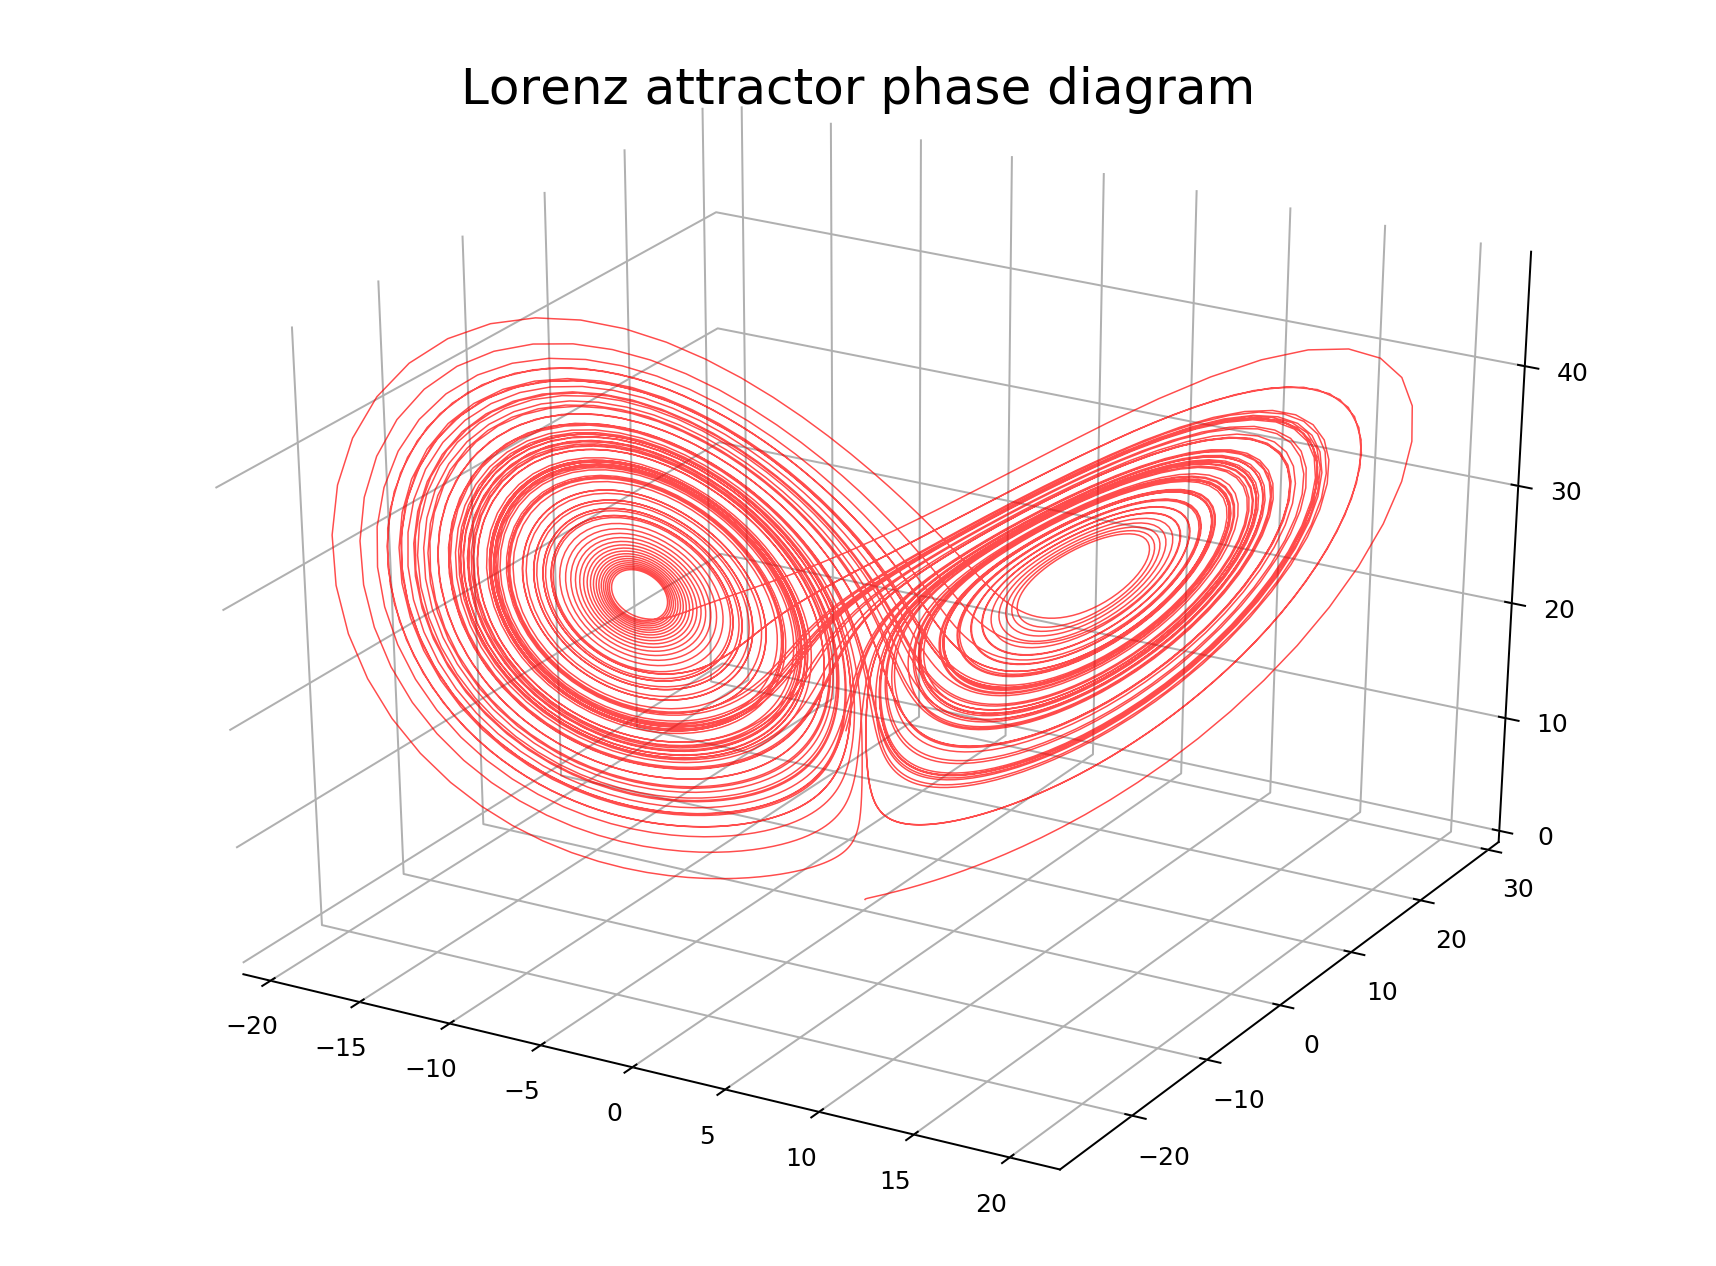
\includegraphics[height=6cm]{lorenz-attractor-3d-1.png}
\end{center}

\begin{center}
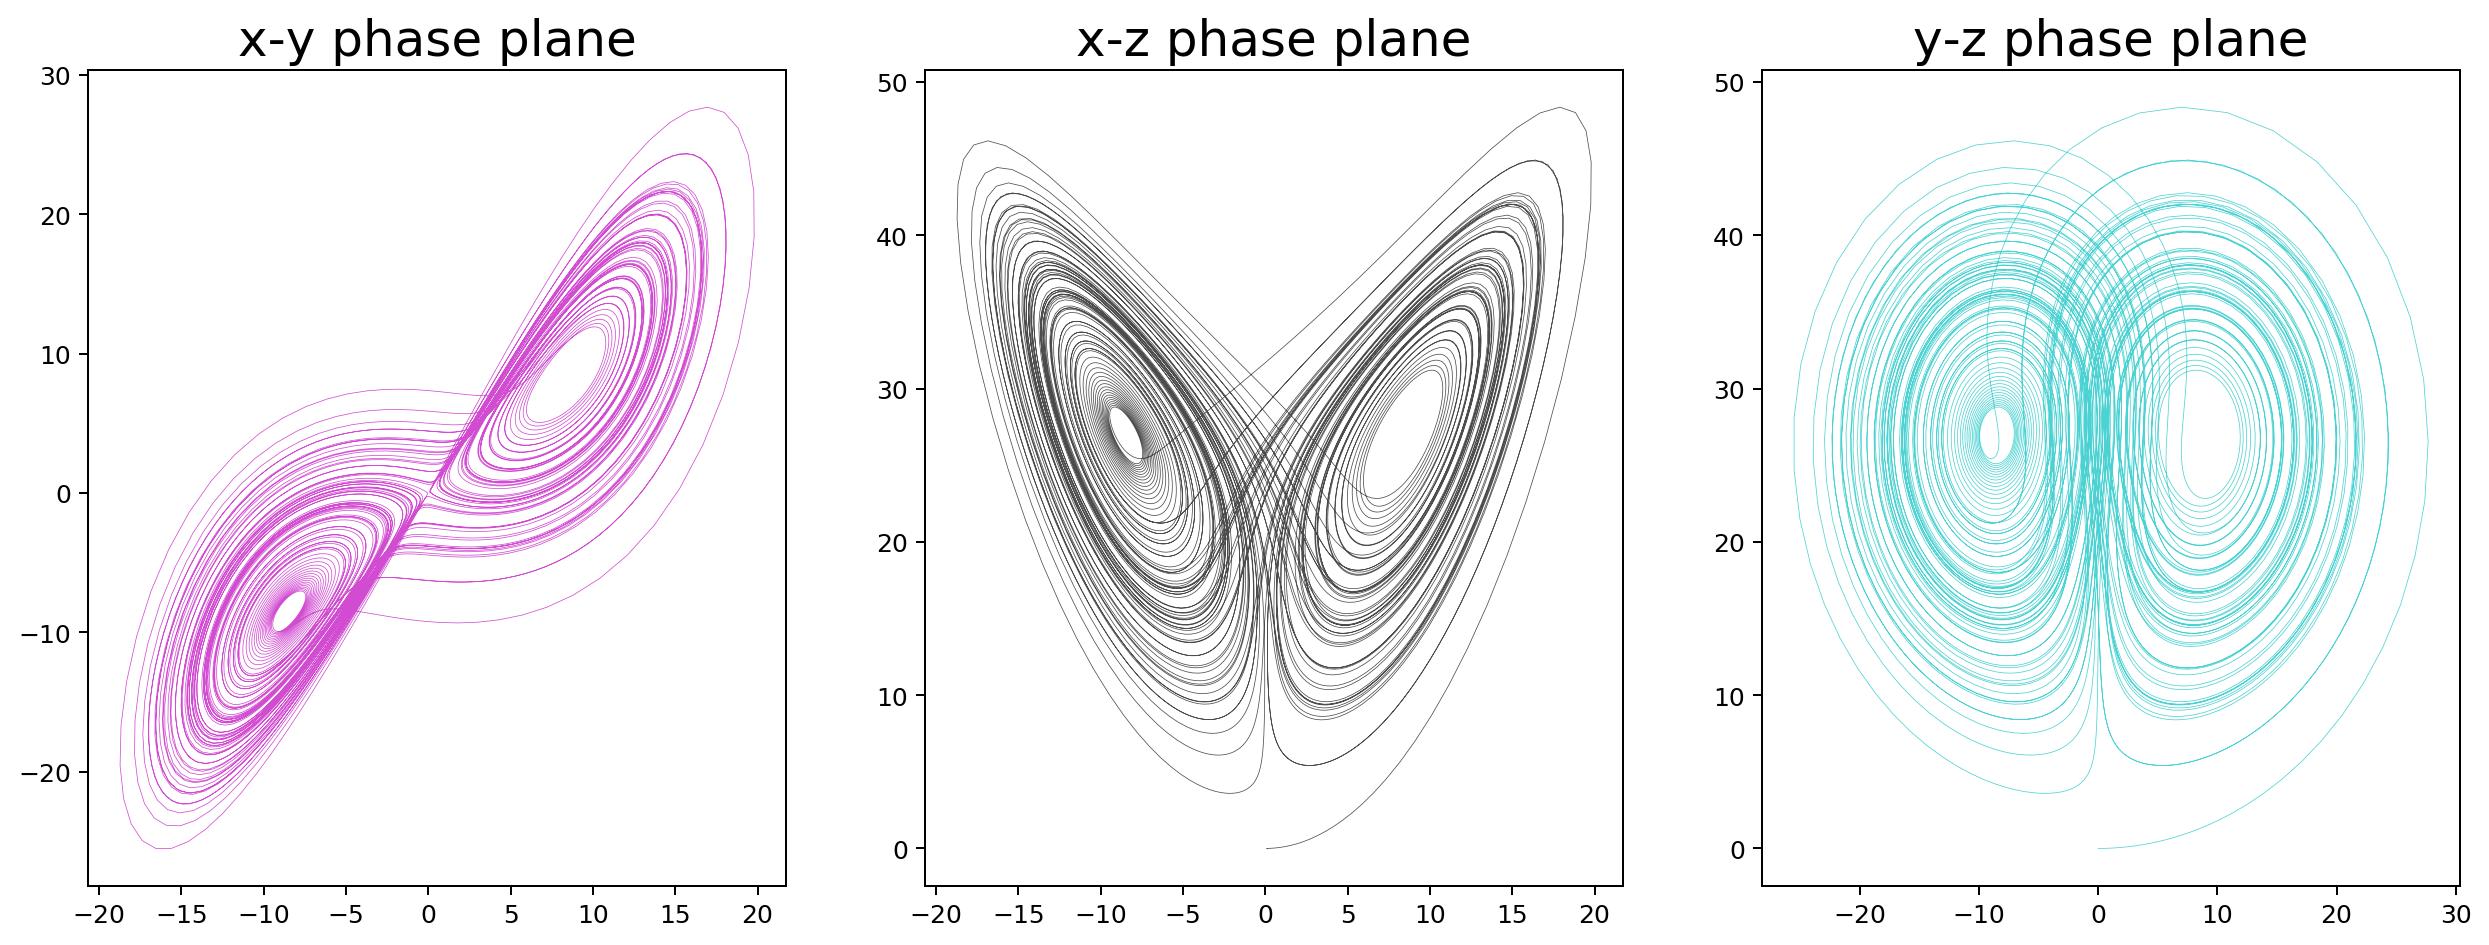
\includegraphics[height=6cm]{lorenz-attractor-phase-plane-1.png}
\end{center}



La animacion del primer punto esta en el respositorio hithub

\vspace{6.5cm}

En el segundo punto se nos pidio realizar las graficas, x(t),y(t),z(t) en un plano bidimensional,para realizar esto nos basamos en la actividad 7 en donde realizamos algo similar, de igual manera utilizamos los arreglos obtenidos de la funcion odeint de las tres varaibles(x,y,z) en funcion del tiempo que en este caso es el time-points y los graficamos con cada una de las variables

\begin{itemize}
\item x vs t

\begin{center}
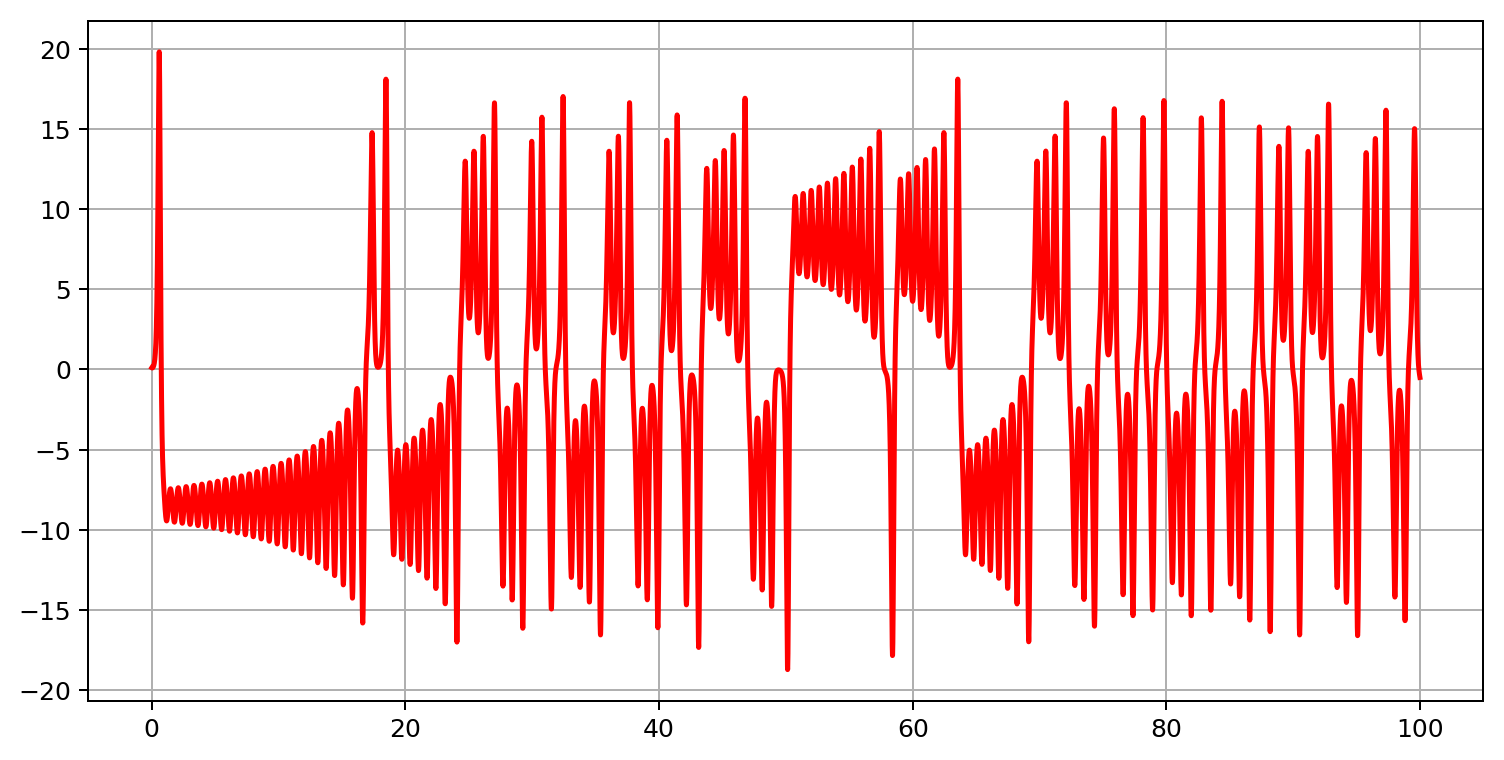
\includegraphics[height=6cm]{x_t.png}
\end{center}

\item y vs t

\begin{center}
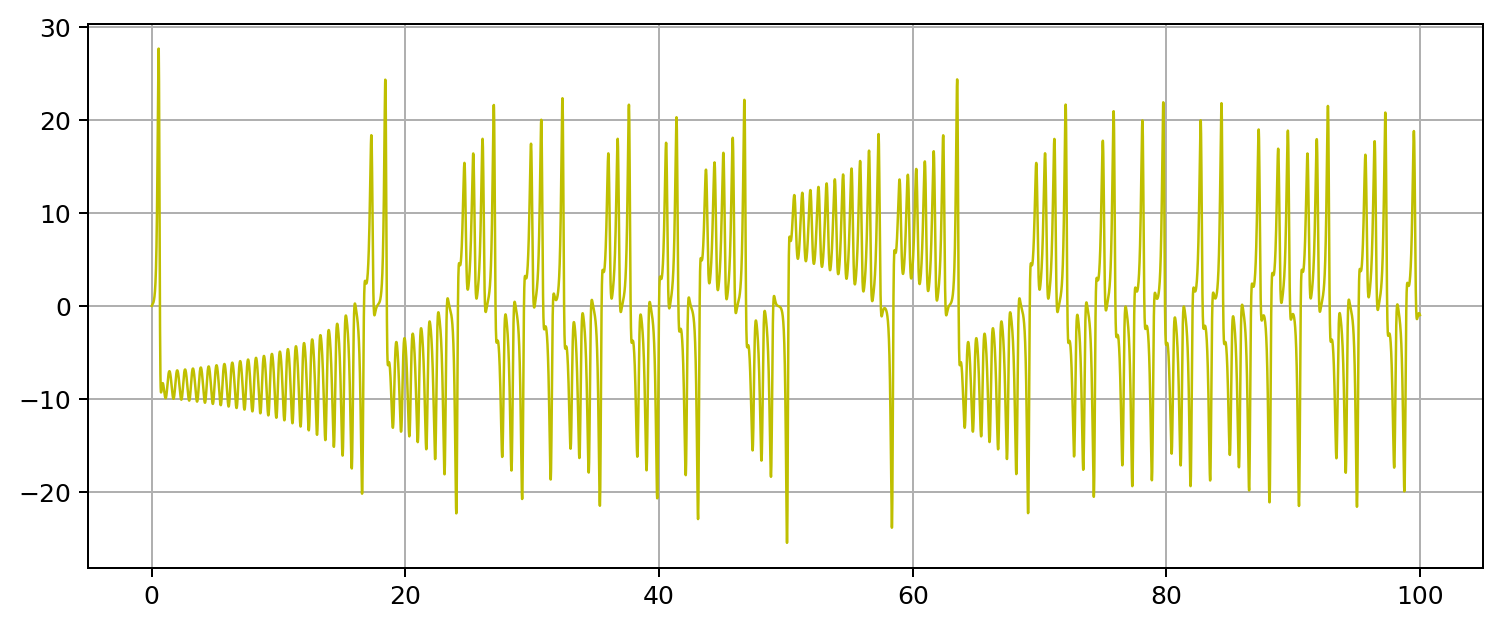
\includegraphics[height=6cm]{y_t.png}
\end{center}

\item z vs t

\begin{center}
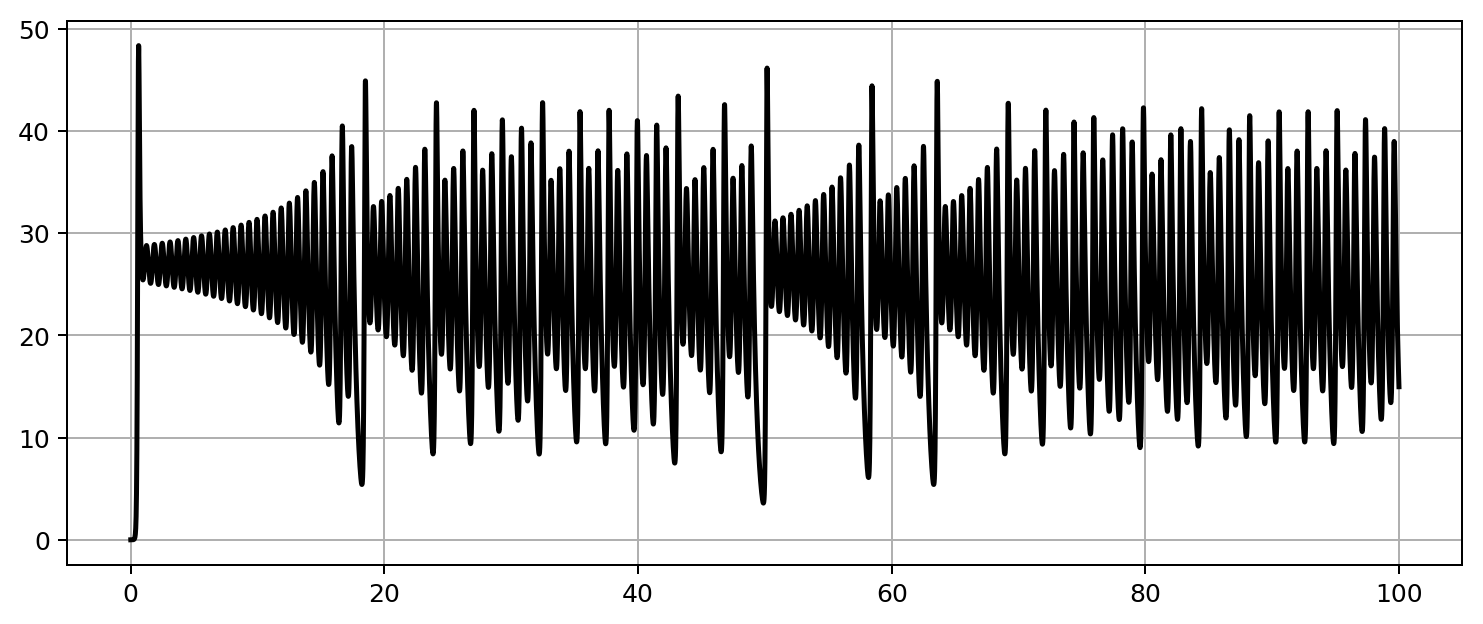
\includegraphics[height=6cm]{z_t.png}
\end{center}

\item xyz vs t

En la imagen siguiente el color, azul corresponde a z, el negro a la x y el amarillo a la y.

\begin{center}
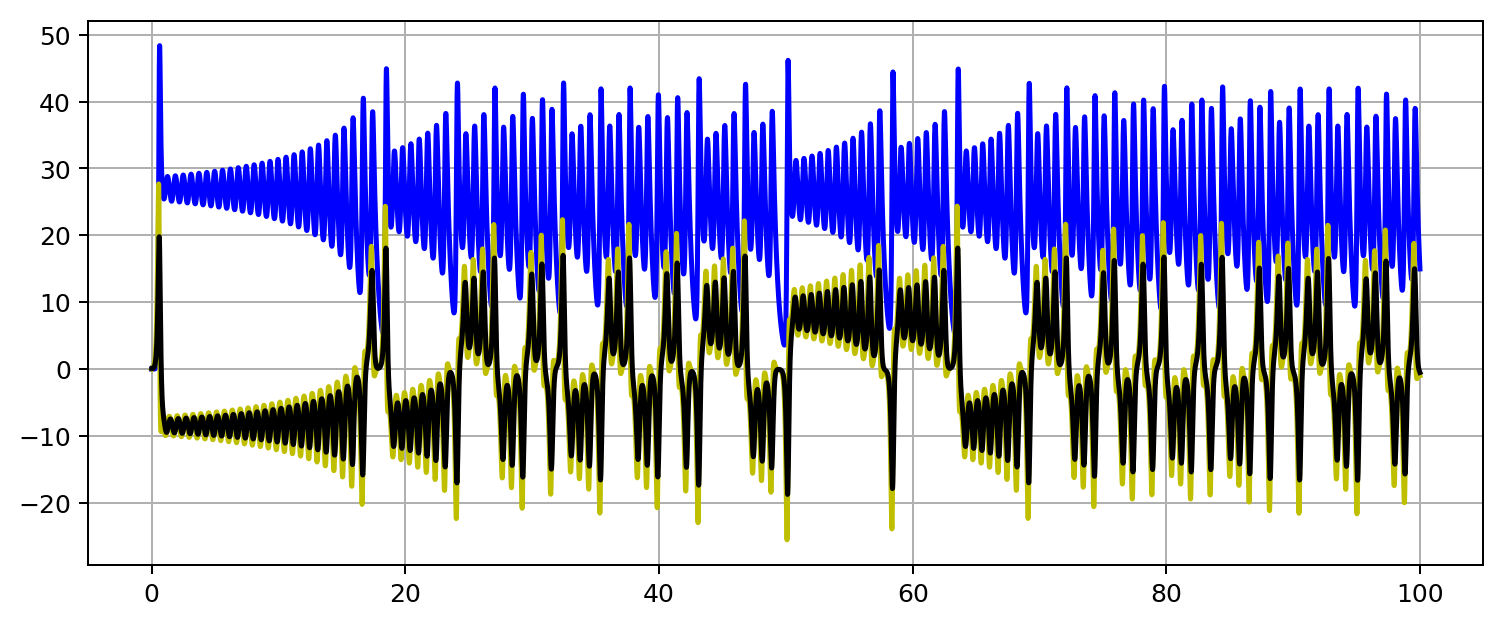
\includegraphics[height=6cm]{xyz_t.png}
\end{center}

\end{itemize}

\vspace{4cm}

El tercer paso es realizar lo mismo que en el paso 1 pero con diferetes valores,los parametros son los siguientes:

\begin{center}

\includegraphics[height=0.5cm]{cod2.PNG}
\end{center}


con los cuales se producieron las siguientes graficas:

\begin{center}
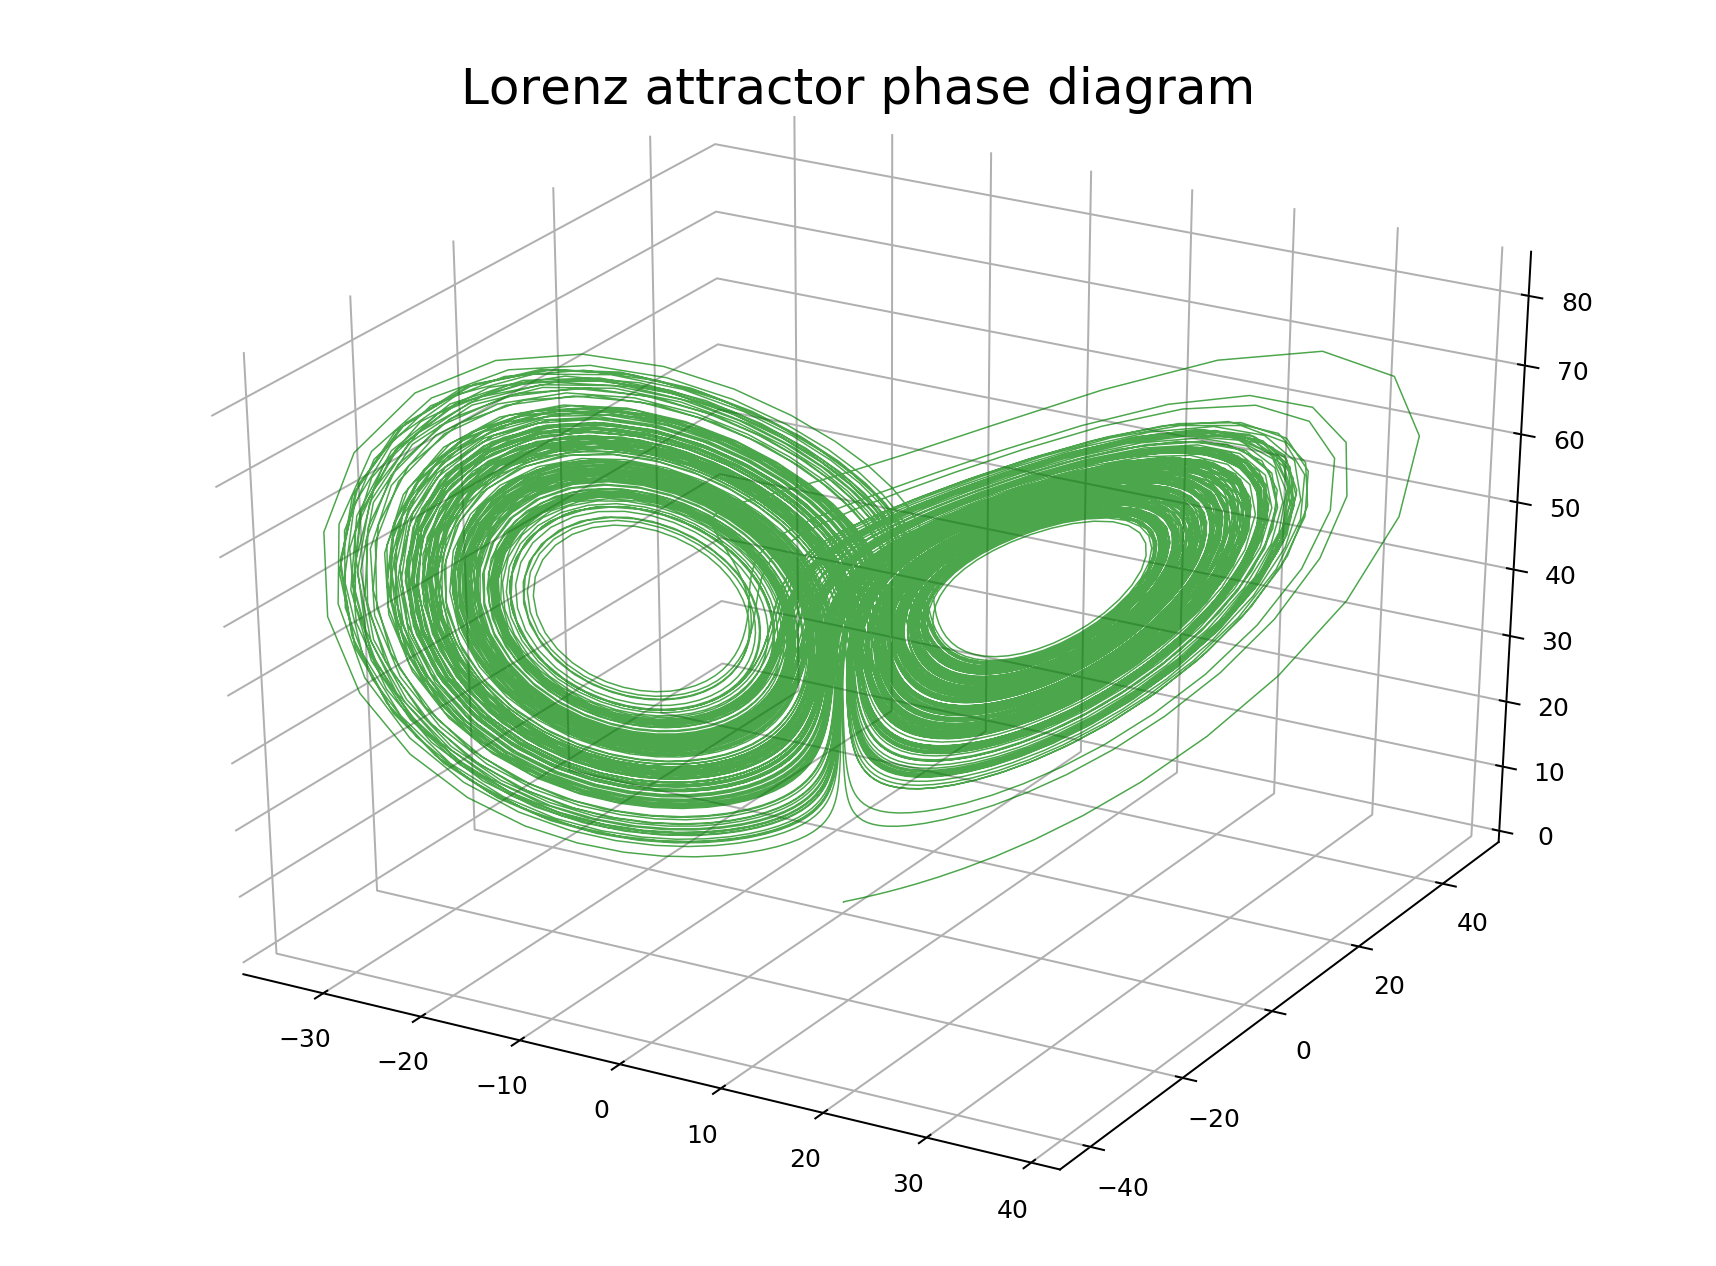
\includegraphics[height=6cm]{lorenz-attractor-3d-3.png}
\end{center}

\begin{center}
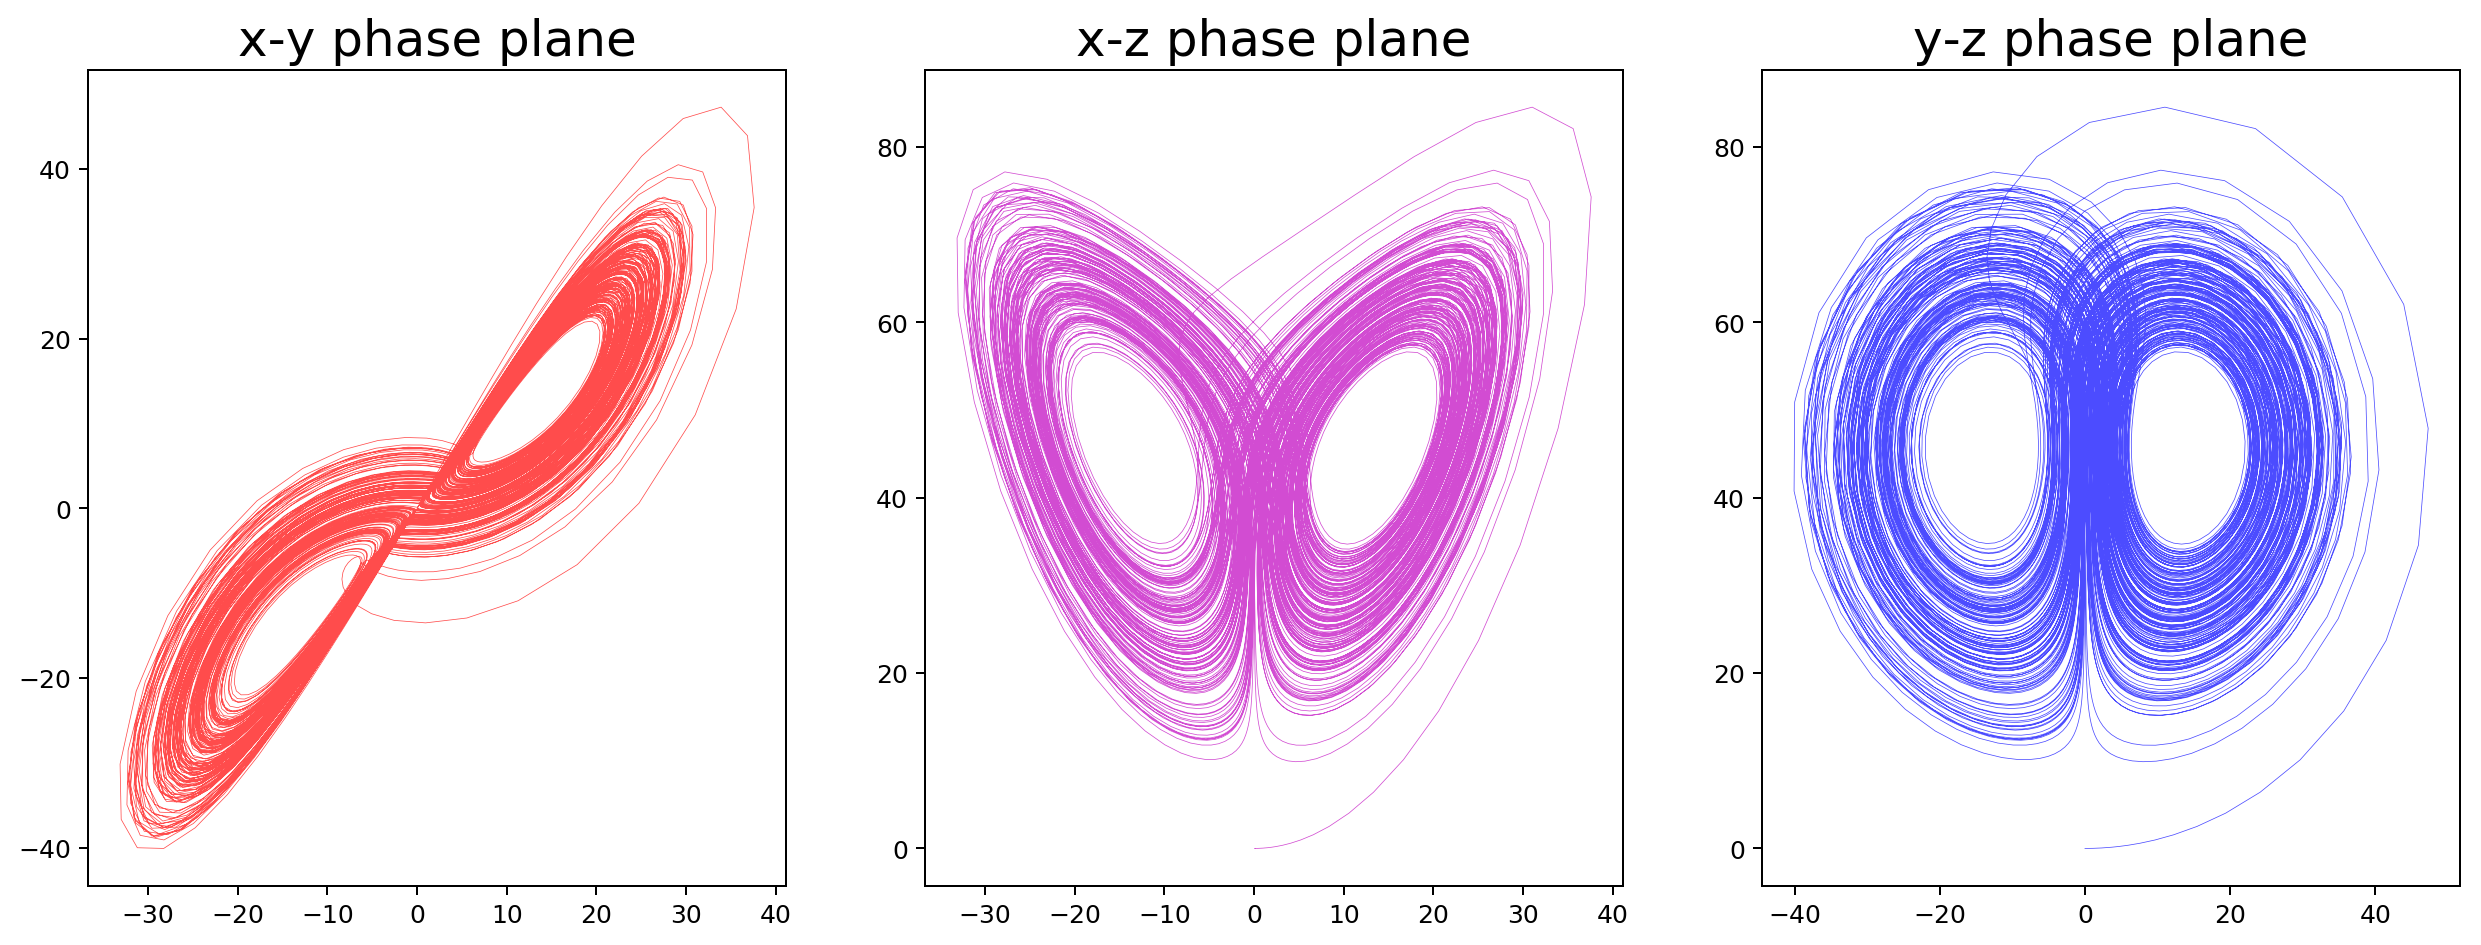
\includegraphics[height=6cm]{lorenz-attractor-phase-plane-3.png}
\end{center}

La diferencia del punto 1 a este punto 4 es que los graficas de los atractores estan mas separados o mas "abiertos sus huecos"

La animacion del segundo punto esta en el respositorio hithub

\vspace{6.5cm}

Este 4to y ultimo paso se llevo acabo lo mismo que en el punto 3 y uno pero de igual manera con diferentes valores de los parametros, esta ves fueron los siguientes:

\begin{center}
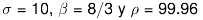
\includegraphics[height=0.5cm]{cod3.png}
\end{center}

con los cuales se llevaron la siguientes graficas:

\begin{center}
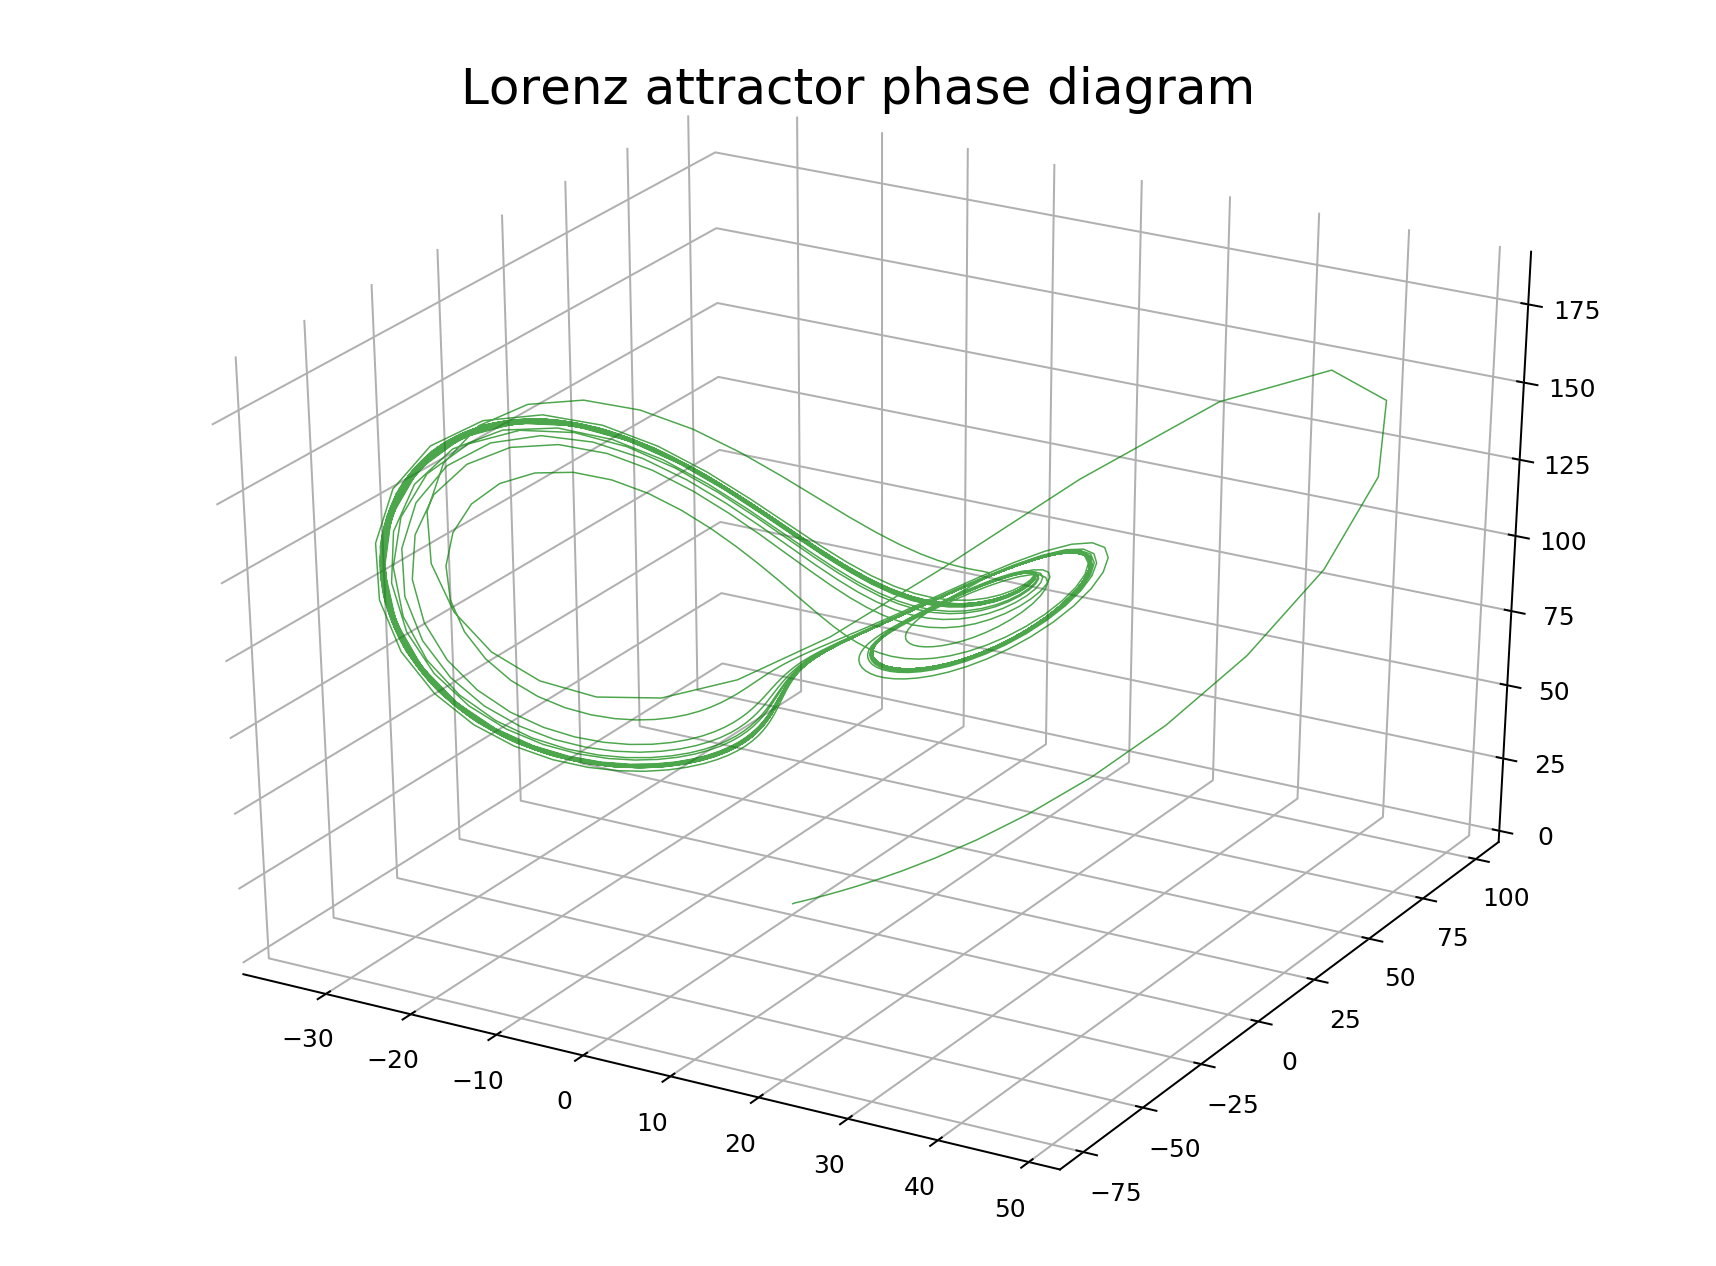
\includegraphics[height=6cm]{lorenz-attractor-3d-4.png}
\end{center}

\begin{center}
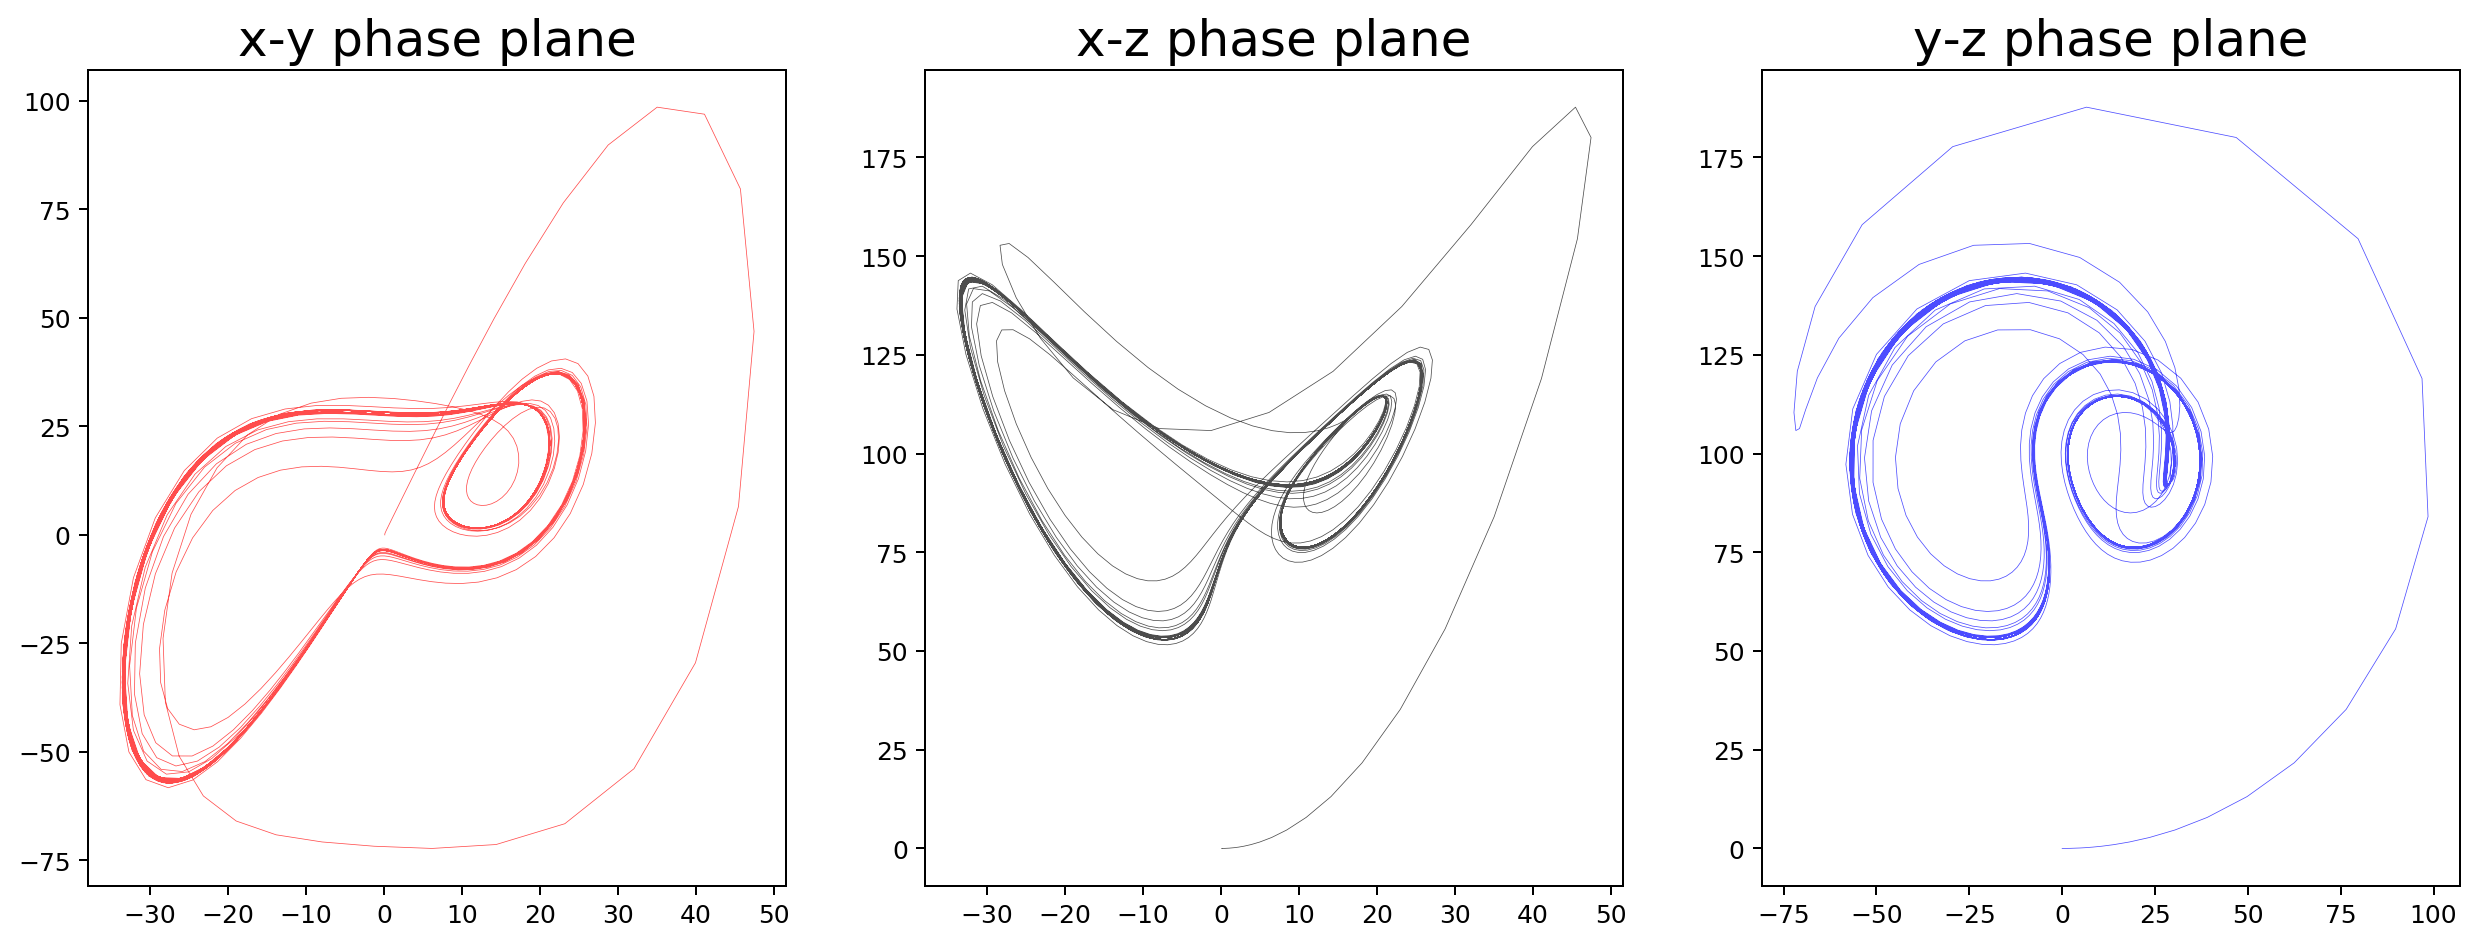
\includegraphics[height=6cm]{lorenz-attractor-phase-plane-4.png}
\end{center}


En estas graficas si se aprecio con mayor facilidad la diferencia debido a que una parte del ocho esta mas "resaltada" o "cerrada" que la otra punta que esta mas "abierta" y tambien se noto que se tarda mas tiempo en llegar al atractor.


\section{Conclusion}

El sistema trabajado Atractor de Lorenz es un sistema que varia mucho es por eso que le llaman caotico, y lo podimos observar en las graficas ya que con el cambio de los parametros cambiamos mucho el atracto, este atractor se utiliza para modelar


Esta evaluación me paracio muy interesante ya que no conocia este es atractor de lorenz y otra observación que cabe recalcar es que se tardan mucho en generar todos los datos y graficarlos.











\end{document}